% !TEX encoding = UTF-8 Unicode
% !TEX spellcheck = en-US


% This is the root file of your thesis: thesis.tex
% A line starting with % is a comment. In some cases, I have included a command preceded by a %. You may activate the command by removing the %.

%%===================================
\documentclass[12pt]{report}
\usepackage{ramsstyle}
\usepackage{parskip}
\usepackage{graphicx}
\usepackage{hyperref}
\usepackage{float}
\usepackage{nth}

%%===================================
%Write the various parts of your thesis as separate files and include them into the main file by the command \include{name of included file}. When you compile the LaTeX file, you may choose which subfiles to include by the command

%\includeonly{chapter01,chapter02}

%%===================================
\begin{document}
% !TEX encoding = UTF-8 Unicode
%!TEX root = thesis.tex
% !TEX spellcheck = en-US

%This is the Titlepage
%%=========================================
\thispagestyle{empty}
\mbox{}\\[6pc]
\begin{center}
\Huge{Investigating the use of Deep Learning for Vectorization of Scanned Raster Maps}\\[2pc]

\Large{Ruben Schmidt Mällberg}\\[1pc]
\large{Fall 2017}\\[2pc]

TBA4560 - Specialization Project\\
Department of Civil and Transport Engineering \\
Faculty of Engineering Science and Technology\\
Norwegian University of Science and Technology
\end{center}
\vfill

\noindent Supervisor 1: Terje Midtbø

\noindent Supervisor 2: Carl Christensen

 % This is the titlepage
\setcounter{page}{0}
\pagenumbering{roman}
% !TEX encoding = UTF-8 Unicode
%!TEX root = thesis.tex
% !TEX spellcheck = en-US
%%=========================================
\addcontentsline{toc}{section}{Preface}
\section*{Preface}
Here, you give a brief introduction to your work. What it is (e.g., a Master's thesis in RAMS at NTNU as part of the study program xxx and\ldots), when it was carried out (e.g., during the autumn semester of 2021). If the project has been carried out for a company, you should mention this and also describe the cooperation with the company. You may also describe how the idea to the project was brought up.

You should also specify the assumed background of the readers of this report (who are you writing for).\\[2cm]

\begin{center}
Trondheim, 2012-12-16\\[1pc]
(Your signature)\\[1pc]
Ola Nordmann
\end{center}
% !TEX encoding = UTF-8 Unicode
%!TEX root = thesis.tex
% !TEX spellcheck = en-US
%%=========================================
\addcontentsline{toc}{section}{Acknowledgment}
\section*{Acknowledgment}
I would like to thank the following persons for their great help during \ldots

If the project has been carried out in cooperation with an external partner (e.g., a company), you should acknowledge the contribution and give thanks to the involved persons.

You should also acknowledge the contributions made by your supervisor(s). 


\begin{flushright}
O.N.\\[1pc]
(Your initials)
\end{flushright}

\subsection*{Remark:}
Given the opportunity here, the RAMS group would recognize Professor Emeritus Marvin Rausand for the work to prepare this template. Some minor modifications have been proposed by Professor Mary Ann Lundteigen, but these are minor compared to the contribution by Rausand.



% !TEX encoding = UTF-8 Unicode
%!TEX root = thesis.tex
% !TEX spellcheck = en-US
%%=========================================
\addcontentsline{toc}{section}{Abstract}
\section*{Abstract}
Old scanned zoning regulations are currently being vectorized using manual techniques in Norway. With the recent advances in image recognition and semantic segmentation using convolutional neural networks, there should be a possibility to use them for automatic vectorization of the regulations thus, lowering the cost and time spent doing manual work.

This paper gives an overview of the state-of-the-art regarding image segmentation using convolutional networks and vectorization techniques for automatic vectorization of raster maps. We also look at how the dataset needed to train a convolutional neural network can be automatically created by using already vectorized zoning regulations.

We show that the current techniques of vectorization need simple raster maps with uniform looks and clear polygons, qualities the zoning regulations do not have, and that the automatic creation of the dataset is not so simple as initially though because of the lack of information about the position of the vectorized polygons within the scanned zoning regulations.
\tableofcontents
\setcounter{page}{0}
\pagenumbering{arabic}

% Better image captions with source.
\newcommand*{\captionsource}[2]{%
	\caption[{#1}]{%
		#1%
		\\\hspace{\linewidth}%
		Source: #2%
	}%
}


\chapter{Introduction}
Vectorization is the task of extracting vector layers from raster maps so that they can be used for further analysis, and is often a time consuming manual process \cite{Worboys2003}. With the vast amount of raster maps available online, we are losing valuable information since we are unable to process them automatically.

 There are a couple of software products on the market today concerning the problem of converting a raster map to a vector image such as GDAL Polygonize \cite{OSGeoa} and R2V \cite{Wu1999}. However, these require either very simple and well-defined polygons or human intervention to successfully vectorize the raster map.
 
 Problems occur when the rasters not only consists of isolated objects that are easy to distinguish but contains a spatial structure, overlapping geometries, and background layers. The multilayered nature of raster maps in addition to varying image quality makes automatic vectorization a hard problem to solve.
 
 Deep convolutional neural networks (DCNN), are top performers of semantic image labeling \cite{Krizhevsky2012} and can, therefore, be a possible solution to the vectorization problem. DCNN require large amounts of properly labeled training data. This is often generated manually for each case with, for instance, crowd-sourcing tools such as Amazon's Mechanical Turk \cite{Krizhevsky2012}.
 
 In this paper, we will look at the state of the art in vectorization of raster maps and image segmentation with DCNN, look at the data needed to train the networks sufficiently and investigate the considerations one would have to take into account when implementing a network.


\chapter{Motivation}\label{chp:motivation }
Digitizing and vectorization is a time consuming and expensive process \cite{Worboys2003}.

In 2009, the Norwegian government made it statutory for all municipalities in Norway to have a digital zoning registers \cite{Kommunaltplanregister2009}. This has many benefits to society, both for the municipalities, the government, and the private sector. Benefits such as faster insights and sped up proceedings for building projects. 

In June 1st, 2017, 354 out of 426 municipalities are registered to have digital zoning registers. The law does however not force the municipalities to vectorize the zoning regulations in detail, only to have them scanned in a digital format such as PDF with the bounding limits of the plan vectorized. The detailed vectorization is then another step that has to be done in order to fully utilize the data in more advanced use cases, such as in GIS. See \autoref{fig:examplezoning} for an example of a zoning regulation in PDF format.

For the municipalities, the digitalization and vectorization is a process that is often done by external contractors. In a project in Telemark and Vestfold, the cost was estimated to be around 3000NOK for each plan, where the whole project consisted of 100 plans \cite{Bo2009}. The cost savings in automating the vectorization of digitized zoning plans are thus economically significant. 

Since the zoning regulations has to follow strict quality standards, the acccuracy of the output from the deep CNN also has to follow these standards. With many zoning regulations already digitized and vectorized, we potentially have a lot of validated, accurate data that can bee used to generate training data for the deep CNN. This gives us a great oportunity to investigate the performance of deep CNNs for vectorization of scanned maps. 

There are a lot of approaches and network architectures that need to be examined and reviewed for this specific problem. This research will be the basis of the author's master thesis, where a practical implementation of the theory found in this research will be done. 


\begin{figure}[H]
	\centering
	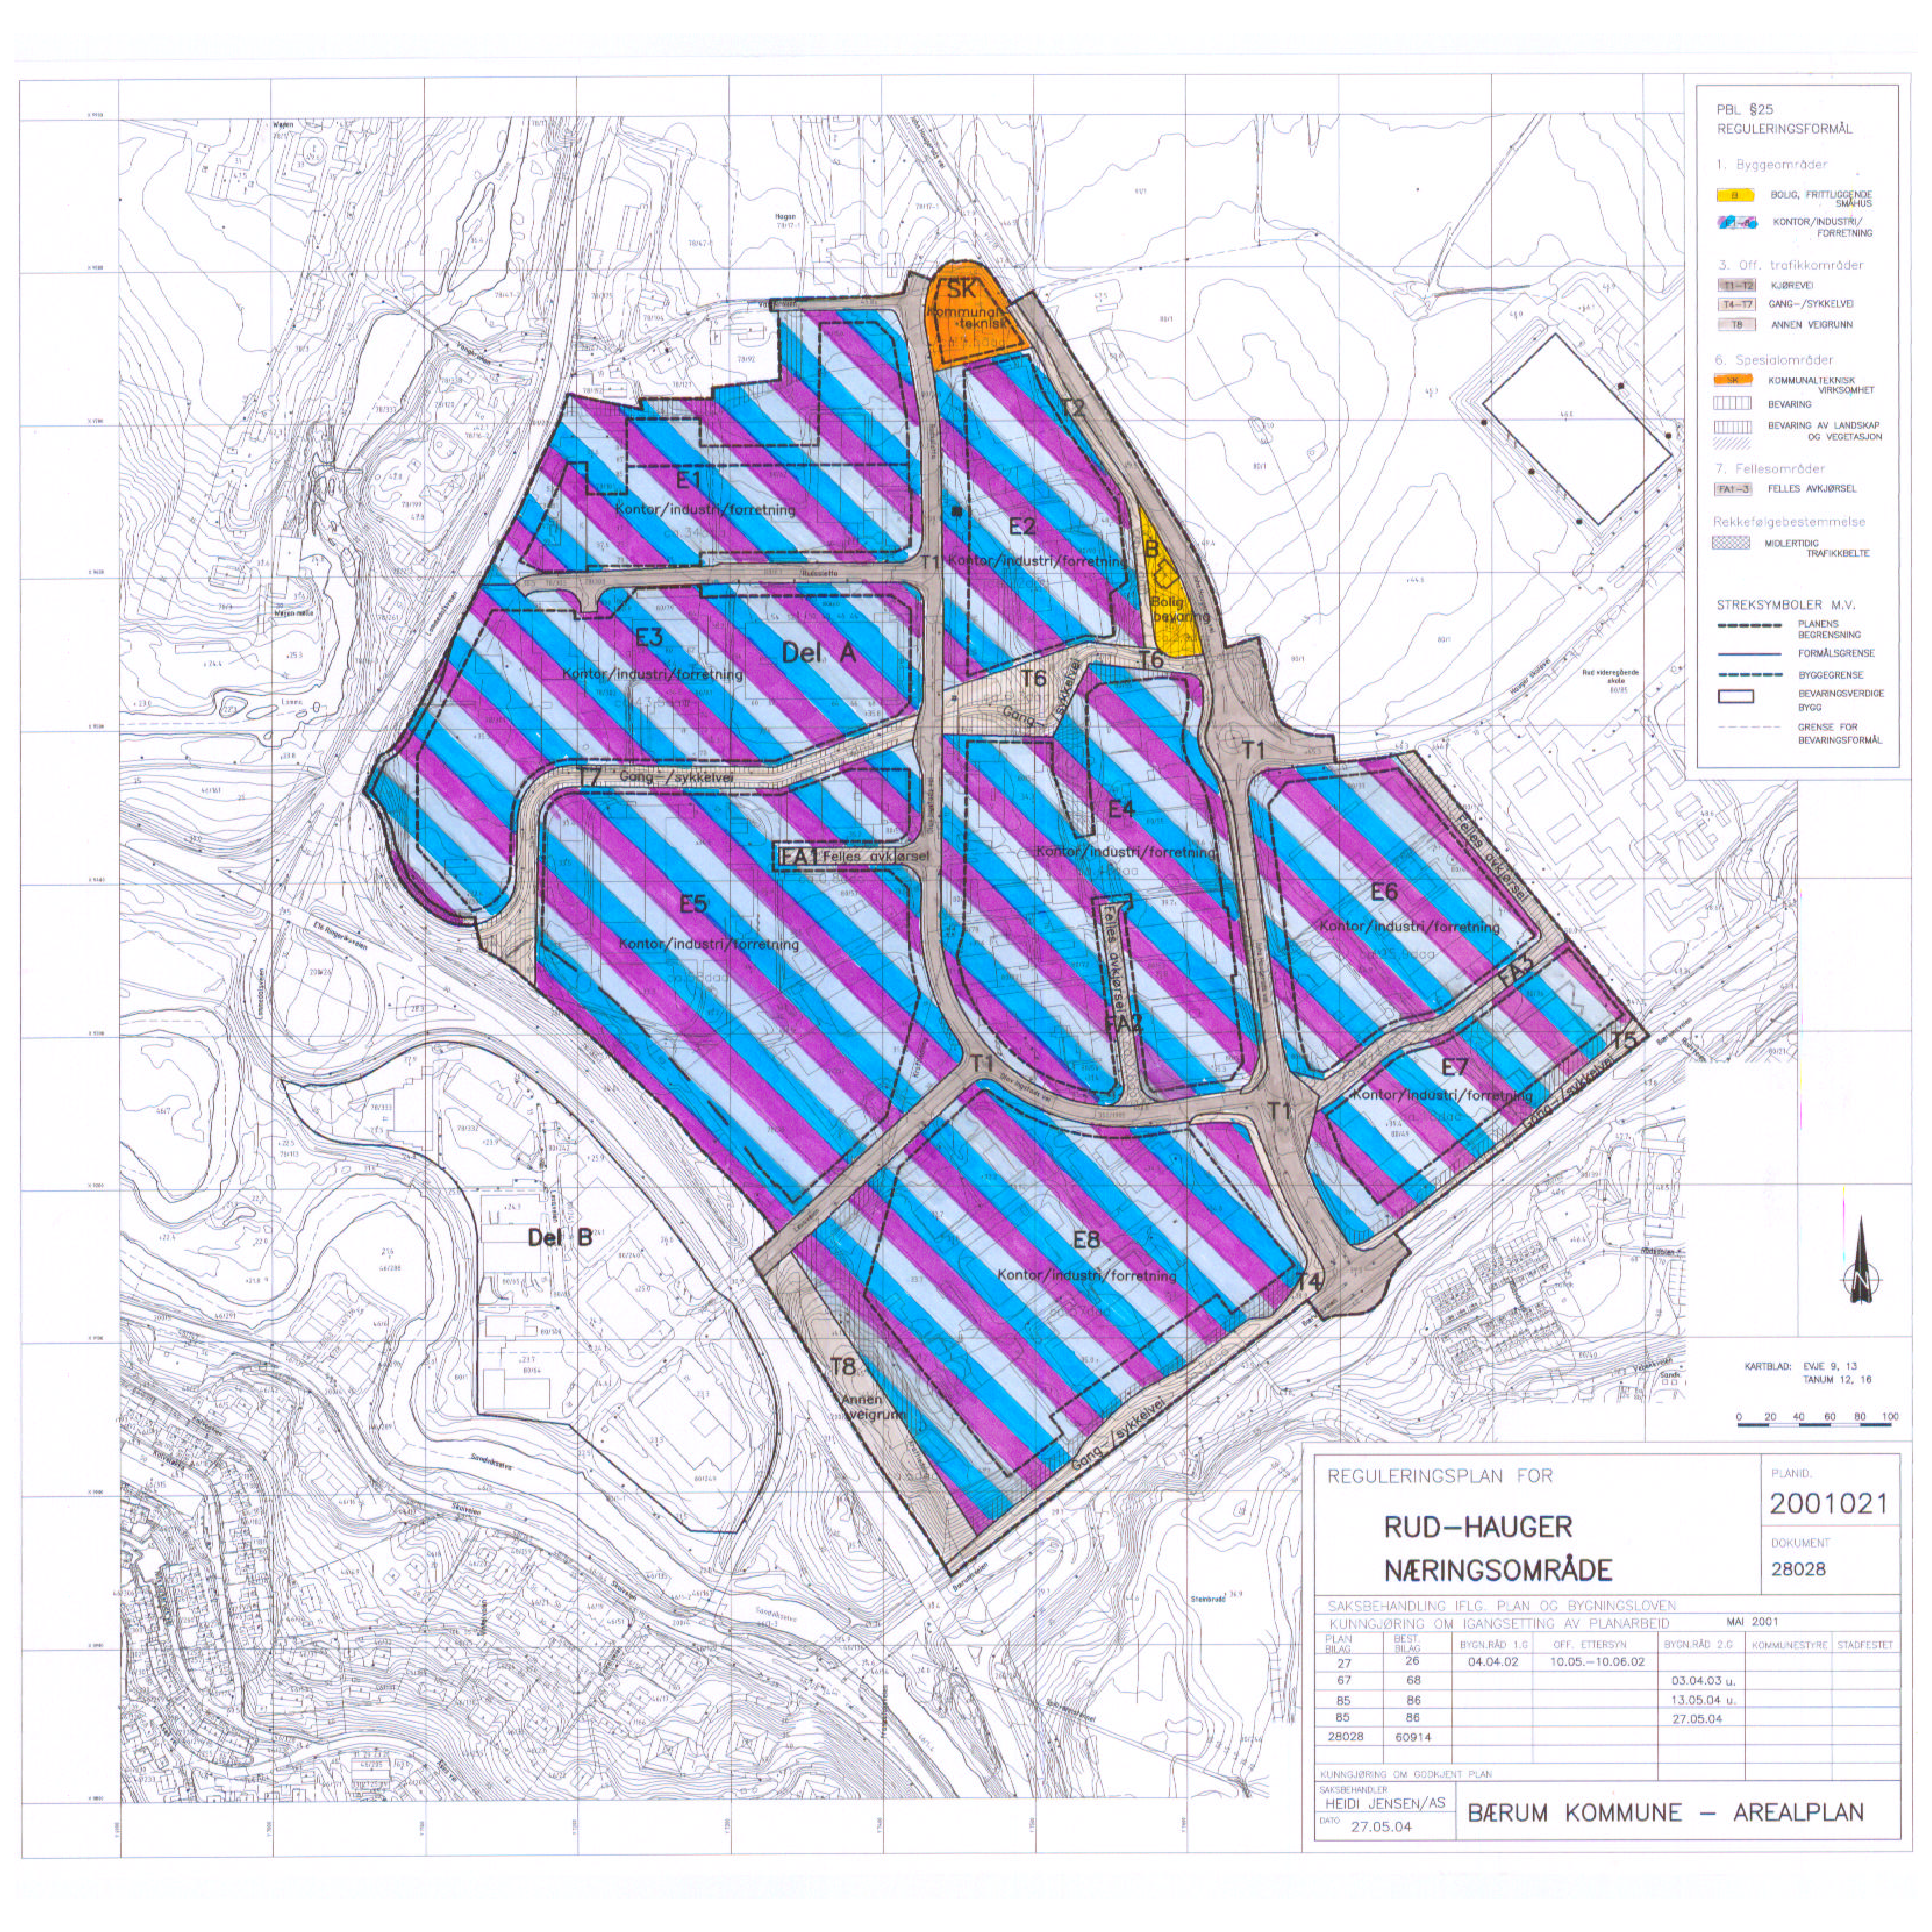
\includegraphics[width=0.8\linewidth]{fig/eksempel_plan.pdf}
	\caption{Scanned zoning regulation in PDF format from Bærum municipality. }
	\label{fig:examplezoning}
\end{figure}

\chapter{Vectorization}\label{chp:vectorization}
Vectorization, raster-to-vector conversion or image tracing is the conversion of raster graphics to vector graphics. To understand the reason for converting from raster to vector we need to look at some of the properties of both storage techniques.

Raster data is structured as an array of grid cells, also referred to as pixels. Each cell in a raster can be addressed by its position in the array, by row and column number. Since each pixel has it's own value, a raster can represent a range of spatial objects. A point can be represented by a single pixel, an arc represented by a sequence of pixels and an area as a collection of continuous pixels. Vector data is structured as a finite straight line segment defined by its endpoints. The location, or coordinates, of the endpoints, are given with respect to a coordinatization of the plane. The vector representation is not discretized in a grid space the same way as a raster but does follow an implicit grid structure as a result of the nature of computer arithmetic. Like the raster, the vector structure can represent multiple spatial structures. A point is given by its coordinates, an arc represented as a sequence of line segments, each consisting of start and end coordinates and an area represented by its boundary consisting of a collection of vectors.

\begin{figure}[H]
	\centering
	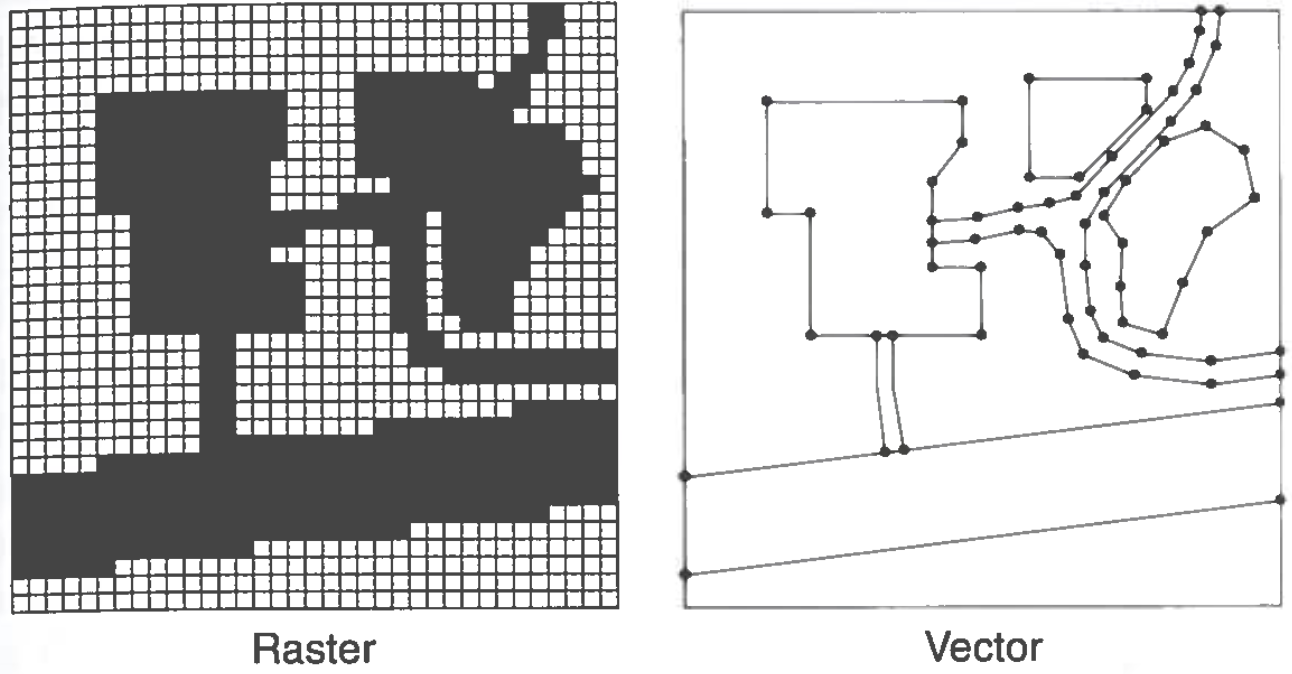
\includegraphics[width=0.8\linewidth]{fig/rastervector.png}
	\captionsource{Raster and vector data}{\cite{Worboys2003}}
	\label{fig:rastervsvector}
\end{figure}

There are multiple reasons for storing data in vector format: The geographic accuracy is higher since it is not dependent on grid size, it allows for efficient encoding of topology, an important aspect when doing analysis that utilizes topologic relations, such as proximity and network analysis, vector data allows for storage of attributes in the data, giving us another dimension of information and the storage size is smaller.

There are multiple different techniques for vectorization. Some of the well known are:

\begin{itemize}
	\item Hough Transform based methods
	\item Thinning based methods
	\item Contour based methods
	\item Run-graph based methods
	\item Mesh pattern based methods
	\item Sparse-pixel based methods
\end{itemize}

All these have different properties and it is important to choose the one that is best for the specific problem. 

\section{Hough Transform}
The Hough Transform can isolate features of particular shape within images. The user must describe the desired feature in a parametric form, therefore the most common application of Hough Transform is to detect regular curves such as lines and circles. The technique is known to be tolerant of image noise and gaps in the feature boundary.

Hough Transform works by transforming each of the pixels into a straight line in a parameter space. The parameter space is described by the parametric form of features we are looking for. In the simplest case of a Hugh Transform, we want to detect straight lines. For this the normal form $r = x cos(\theta) + y sin(\phi)$ is used to represent the lines. When iterating the pixels in the image the algorithm looks if there is enough evidence that there is a straight line at that pixel, if there is, it calculates the parameters $\theta$ and $\phi$ at that point and adds it to an array. The array accumulates all the points that belongs to each specific $\theta$ and $\phi$, thus the more points that are on the same parameters the more likely they belong to a line. The algorithm visits each pixel one time and is therefore linear with the number of pixels in the image.

\section{Thinning}
Thinning is a morphologic operation that is used to remove foreground pixels from an image, resulting in a simplified image with the same topologial relations as the input image. It works by successively removing pixels from the boundary until there is not possible to remove more. The skeleton that is left contains the centerlines of the objects. This technique is mostly used on binary images. The iterative nature of the algorithm makes it computationally expensive.

\section{Contour}
This method aim at lowering the computational cost compared to thinning. The main idea is to find edges before calculating the middle point that is between two opposite parallel edges. A chain of middle points represent the medial axis. It has to use a edge detection algorithm before extracting the middle points between the edges. A problem with the contour based methods is how they deal with junctions. It is likely to miss junctions that are crossing at a small angle and it has difficulties with cross intersections where four lines meet \cite{Wenyin1999}. It is thus not suited for vectorization of curves and crossing lines.

\section{Run-graph}
Run-graph is a semi-vector representation of the raster image \cite{Monagan1993}. It examines the raster in either row or column direction in what is defined as horizontal and vertical \emph{runs}. A horizontal run is a maximal horizontal sequence of black pixels. A vertical run is a maximal vertical sequence of black pixels. After running, the run-graph is composed of edge areas that represent line segments and node areas and touching points that correspond to endpoints and junctions. The line extraction from the graph attempts to minimize the area of the node and maximize 

\section{Mesh pattern}

\section{Sparse-pixel}

\chapter{Image segmentation with Deep Learning}
In this chapter, we will look at the problem of image segmentation and the state of the art regarding segmentation and object detection using Deep Learning. We will look at both semantic and instance segmentation.

Semantic segmentation of images is one of the key problems in the field of computer vision. It is about making dense predictions inferring labels at the pixel level, assigning a class to each pixel with its enclosing object \cite{Garcia-Garcia2017}. Taking it a step further, we get to instance segmentation, where we want to associate the classes with a physical instance of an object. 

Both semantic and instance segmentation can be seen as giving us an understanding of an image at a higher level. This fine-grained control of an image greatly helps with scene understanding which is becoming more and more relevant with the increasing number of applications, such as self-driving cars and augmented reality. 

We can see an example in \autoref{fig:segmentation} where we see the difference between the two approaches. In the middle photo, all the chairs have the same classification, as chairs. In the right photo, we see that the chairs now are classified as chairs, but with a different class for each of them. We can see that instance segmentation is the combination of both object detection and semantic segmentation.

\begin{figure}[H]
	\centering
	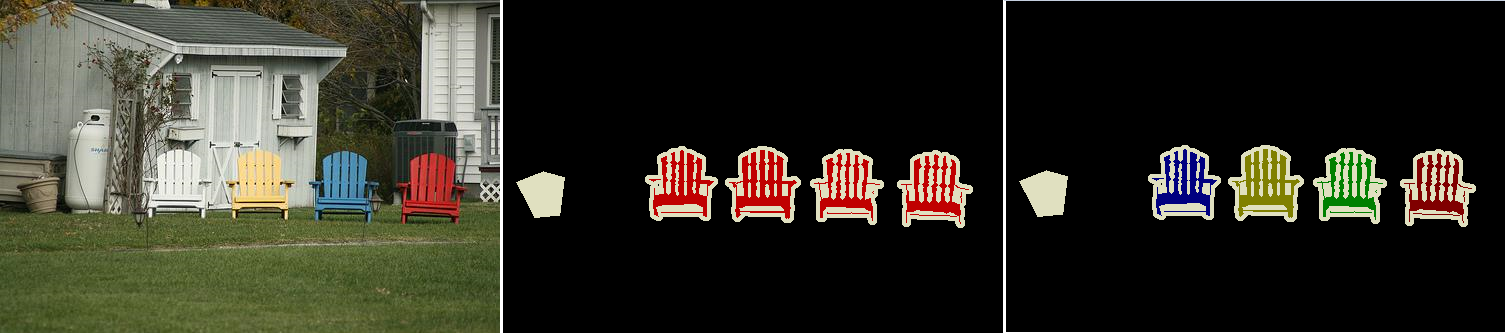
\includegraphics[width=0.8\linewidth]{fig/se.png}
	\caption{Left: input image. Middle: Semantic segmentation. Right: Instance segmentation. \cite{PASCALVOC2012}}
	\label{fig:segmentation}
\end{figure}


\section{Neural networks}
To get a deeper understanding of how neural networks perform segmentation of images, we need to take a look at the fundations behind them and how they operate.

Neural networks are a computational model that shares som properties with the animal brain in which simple units called neurons are working in parallel with no centralized control unit \cite{Patterson2017}. The primary means to long-term information storage is in the weights between the units and updating them is the primary way the network learns new information.

A network is defined by the number of neurons, number of layers and the connections between the layers. One of the easiest architectures to understand is the feed-forward multilayer architecture viewed in \autoref{fig:feed-forward}. It is a neural network with an input layer, one or more hidden layers and an output layer. The input layers feeds input, in the form of vectors, to the rest of the network. The number of neurons at the input layer often reflects the size of the input vector.

\begin{figure}[H]
	\centering
	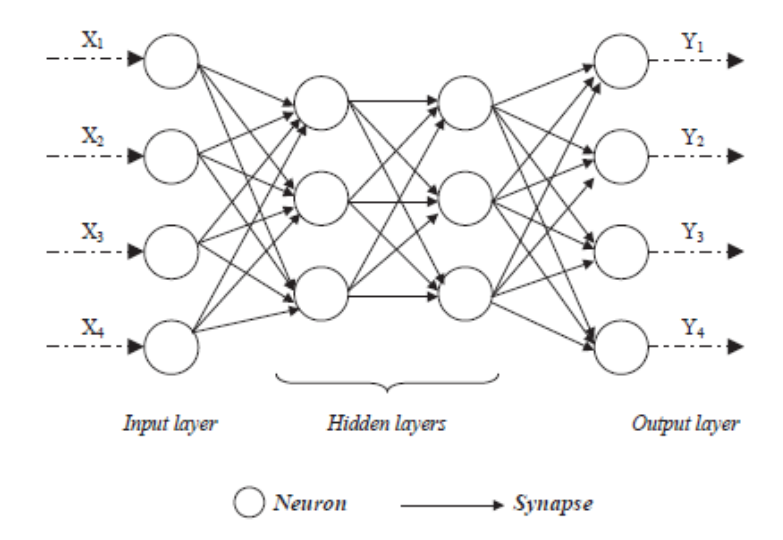
\includegraphics[width=0.6\linewidth]{fig/feedforward-neural-network.png}
	\caption{Structure of a multilayer feed forward network. \cite{Zangeneh2011}}
	\label{fig:feed-forward}
\end{figure}

\subsection{Artificial neurons}
Each layer consist of one or more artificial neurons, also called nodes. An artificial neuron is a mathematical representation of a biological neuron and consist of inputs with weights and bias, a transfer function and an activation function. The weights are what scales, either amplifying or decreasing, the input to the node. The bias is a constant scalar value per layer that is added to ensure that at least some of the nodes in the layer are activated, that is, forwarding a non-zero value to the next layer. The transfer function takes the weighted sum of the input variables and transfers it to the activation function. The activation functions are scalar-to-scalar functions that defines the output of the node based in the inputs, weights and bias. A model of an artificial neuron compared to a real one, can be seen in \autoref{fig:artificial-neuron}. 


\begin{figure}[H]
	\centering
	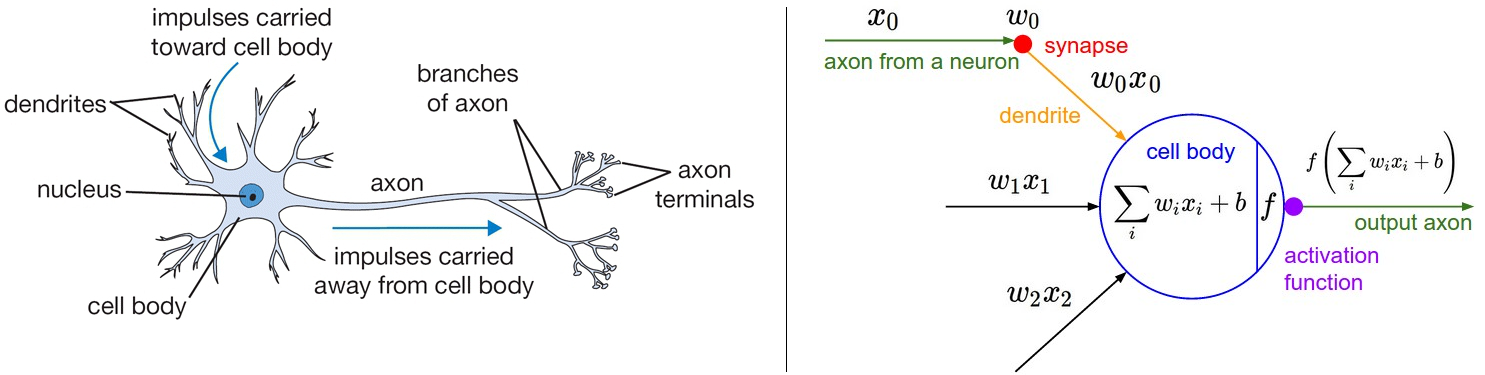
\includegraphics[width=\linewidth]{fig/artificial-neuron.png}
	\caption{Structure of a real neuron compared with an artificial one. \cite{Li}}
	\label{fig:artificial-neuron}
\end{figure}

\subsection{Activation functions}

The use of activation functions in the hidden layers add the ability for the network to learn non-linear functions. We will now take a look at some of the usefull activations functions that are used today.

\subsubsection*{Sigmoid}
The sigmoid activation function has a characteristic "S"-shaped curve and can take variables of near infinite range and convert them to values between 0 and 1. It is good at reducing outliers and extreme values in the dataset. Expressed mathematical as:

\begin{equation}
a = \sigma(x) = \frac{1}{1+\exp(-x)}
\end{equation}


\subsubsection*{Tanh}

A trigonometric hyperbolic function. Tanh can normalize input to the range of -1 to 1 and can therefore deal with negative numbers better than the Sigmoid. Expressed mathematically as:

\begin{equation}
a = \sigma(x) = \tanh(x)
\end{equation}


\subsubsection*{Rectified Linear}

Rectified Linear only activates a node if it is above some threshold. When the input raises above the threshold it has a linear relation to \autoref{eq:relu}. Nodes that use the rectifier are called Rectified Linear Unit or ReLU. 

\begin{equation}
\label{eq:relu}
a = \sigma(x) = \max(0, x)
\end{equation}


ReLUs are the state-of-the-art because of their proven usefulness in many situations and their ability to train better in practice than sigmoids. ReLU does not have the so-called problem of vanishing gradients either. Vanishing gradients is a problem that occurs when using gradient-based methods (explained in \autoref{subsection:backprop}) for learning, where large changes in the value of parameters from the early layers, does not have a big effect on the output, making the network lose its ability to learn. The reason for this happening is that some activation functions, such as sigmoids or tanh, forces the input space into small regions. 

While removing the problem of vanishing gradients, ReLU introduces another one and that is the problem of "dying ReLU" \cite{Li}. This is a problem that occurs when a large gradient passes through the neuron causing the weight update to be so large that it causes the neuron to never activate again, that means that the gradient passing through the neuron will be forever zero.


\subsection{Training}
There are different forms of learning such as supervised, where we show the network what the correct answer is. Unsupervised, where the network itself decides how to label the data and reinforcement learning, where the network does not get to know the answer but learns by reward or punishment. We will only focus on supervised learning in this paper as this is the type of learning we use when doing image segmentation.

In supervised learning, the network learns by training on a set of inputs and desired outputs. As inputs are passed through the network and outputs are generated, it learns by adjusting weights and biases causing some neurons to become smaller and some to become larger. The larger a neuron's weight is, the more it affects the network and vice versa.

By adjusting the weights and biases, the network reduces the errors, also called loss. The loss is defined by some loss function that quantifies the correctness of the output from the network in regards to the ground truth. By using a loss function we reclass the learning problem as an optimization problem, where we try to minimize the loss.

The most common algorithm for the weight adjustment in neural networks is called \emph{backpropagation}.


\subsubsection*{Backpropagation Learning}\label{subsection:backprop}
When the output from a neural network produces a large loss, we need to update the weights accordingly. A problem with multilayer neural networks, however, is that there are many weights connecting an input with an output, so it becomes difficult knowing what weights that affect the output. We need a clever way of finding what specific weight that contributes to the output. This is the problem backpropagation tries to solve. A high level understanding of backpropagation is that we use the chain rule to iteratively calculate the gradients for each layer. The steps of the algorithm is as follows:

\begin{enumerate}
	\item Initialize network with random weights
	\item Loop trough the training examples
	\item Compute the network output for the current training example
	\item Compute the loss with the loss function.
	\item Compute the weight update for the output layer with the weight update rule:
	$$
		W_{j,i} \leftarrow W_{j,i} + \alpha \times \alpha_j \times \Delta_i
	$$
	
	Where 
	$$
		\Delta_i = Err_i \times g'(input\_sum_i)
	$$
	
	and $g'$ is the derivative of the activation function
	
	\item Loop trough all the layers in the network all the way to the input layer and:
	\item Compute the error at each layer with the propagation rule:
	$$ 
		\Delta_j \leftarrow g'(input\_sum_i)\sum_{i}W_{j,i}\Delta_i
	$$
	
	\item Update the weights leading in to the hidden layer with the update rule:
	
	$$ 
		W_{k,j} \leftarrow W_{k,j} + \alpha \times \alpha_k \times \Delta_j
	$$
	
\end{enumerate}

The term $\alpha$ is the learning rate, and belongs to the family of what we call \emph{Hyperparameters} in machine larning.

\subsubsection*{Hyperparameters}
The hyperparameters are what we tune to make the network train faster and better. The selection of these parameters are done to ensure that our network does not \emph{overfit} or \emph{underfit} the data. We say that our model is overfitted if it fits our training data too well but does not generalize enough over the entire dataset. We say our model is underfitted if it generalizes too much and is not able to fit the training set. The terms are illustrated in \autoref{fig:overfit-underfit}. In the left image we see that the model does a bad job at approximating the function, it is underfitted. In the middle image we see that the model approximates the function well. In the right image we see that the model fits the training samples very good, but does a bad job at approximating the function, the model is overfitted.

\begin{figure}[H]
	\centering
	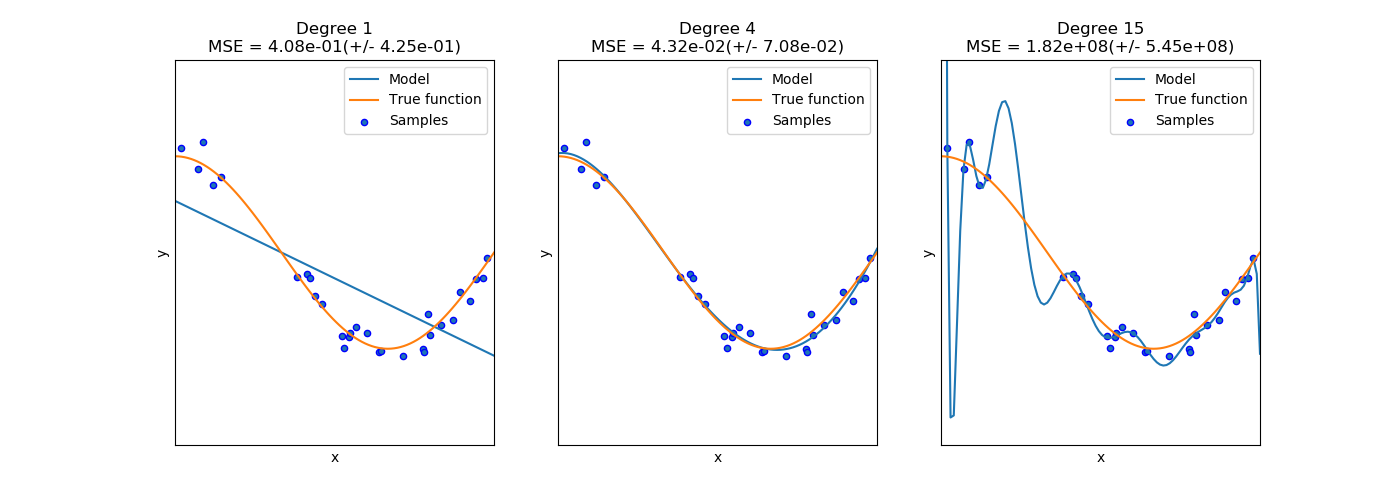
\includegraphics[width=\linewidth]{fig/overfit-underfit.png}
	\caption{Left: Underfitted model. Middle: Appropriate fit. Rigth: Overfitted model. }
	\label{fig:overfit-underfit}
\end{figure}
The learning rate affects the amount we adjust the parameters during training. A large learning rate will make our parameters take large steps, thus saving time, but can cause us to overshoot the minimum of our loss function causing us to never find a minimum. A small learning rate causes us to take smaller steps and should help us reach the minimum, but can take a very long time to do so.

Another important hyperparameter is \emph{regularization}. Overfitting often occurs when some weights have become very large and regularization is about reducing the effects of the large weights in the network. The perhaps most common form of regularization is L2 and is often implemented as the term $\frac{1}{2}\lambda w^2$ that we add to the weights \cite{Li}. Another regularization, introduced in \cite{Srivastava2014} is \emph{dropout}. Dropout works by randomly dropping some of the neurons during training causing it to train on a "thinned" version of the net. Dropout has shown  major improvements over other regularization tehniques \cite{Srivastava2014}.

\section{Convolutional neural networks}
Fully connected multilayer neural networks take inputs as a one-dimensional vector. When using an image as input, these vectors become very large. The reason for this is that we represent each pixel in the image as one value in the vector. If we are working with color images represented with 3 channels of RGB information, each of these also needs to be mapped. For a single 200x200 image this means $200 \times 200 \times 3 = 120000$ connections in only the first layer. This illustrates how bad the fully connected neural networks scale.

Convolutional neural networks, or CNNs, tackle the scaling problem by assuming inputs as images and model them as three-dimensional objects with image width, image height and color channels as the dimensions. At a high level, the architecture consist of an input layer, convolutional layers, pooling layers and fully-connected layers \cite{Patterson2017}. 

\subsection{Convolutional layers}
The convolutional layers, or CONV layers, are the core building blocks of a CNN. The layers consist of a set of learnable filters also called kernels. Each of the filters are small in regards to width and height but are always the same size as the input in regards to depth. The filter is applied to the input by sliding, or \emph{convolving}, the filter accross the width and height of the input. At each position, the dot product between the filter and the input is calculated. The output is a two dimensional map that is called \emph{activation map}. This process is illustrated in \autoref{fig:convolution}. For each of the filters in the CONV layer we get such a map and stack them in the depth direction, this in turn represents the output of the layer. 

\begin{figure}[H]
	\centering
	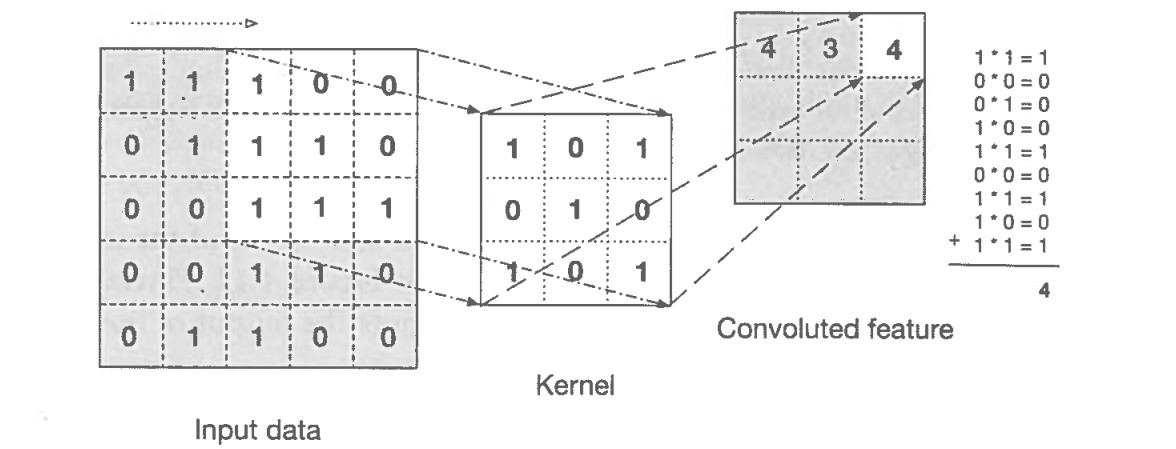
\includegraphics[width=\linewidth]{fig/convolution.png}
	\captionsource{The convolution step.}{\citeauthor{Patterson2017}\cite{Patterson2017}}
	\label{fig:convolution}
\end{figure}

The network will learn filters that causes the node to activate when certain visual features are seen, for instance an edge. Deeper into the network we will se filters that become more global in term of the input and recognizes nonlinear combinations of features. An example of what the filters look like in a deep CNN can bee seen in \autoref{fig:filters} where we see filters learned in the first convolutional layer in an eight layer network \cite{Krizhevsky2012}.

\begin{figure}[H]
	\centering
	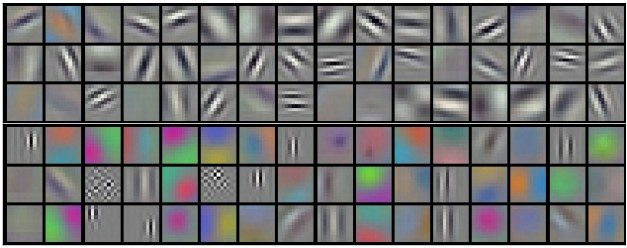
\includegraphics[width=\linewidth]{fig/filters.png}
	\captionsource{96 learned filters in the first convolutional layer. }{\citeauthor{Krizhevsky2012}\cite{Krizhevsky2012}}
	\label{fig:filters}
\end{figure}
%  Local connectivity
If we imagine that we freeze the filter as it is convoluted accross the input, a single step and its calculation, can be viewed as the output from a neuron. The activation map then represents a sheet of neurons with each of the neurons looking at a small part of the input, not knowing anything about the rest of the image. This feature is called \emph{local connectivity} and is an important part of how the network keeps the number of parameters smaller then a regular neural network. All the neurons in the sheet also share parameters, since it is the same filter that did the calculation. This is the concept of \emph{shared paramters} and is the other important part of how CNNs keep the number of paramters low.

\subsection{Pooling layers}
Another way to reduce the number of parameters in the network, is the use of pooling layers. Pooling layers essentially reduces the input size by downsampling the input with different pooling functions. The most common operation is \emph{max pooling} with a 2x2 filter with a stride of 2 that reduces the size by two in the height and width dimension \cite{Li}. 























\chapter{Related work - Image segmentation}\label{sec:previous-work-segmentation}
In this chapter, we will look at some of the previous work done in the field of image segmentation with neural networks. 

During the last ten years, we have seen many important advances when it comes to the architecture of deep networks for image segmentation. AlexNet \cite{Krizhevsky2012}, VGGNet \cite{Simonyan2014a}, GoogLeNet \cite{Szegedy2014}, ResNet \cite{He2015}, ReNet \cite{Visin2015} and the very recent CapsNet \cite{Sabour2017} are all examples of such advances. In the next section, we will look at the main points from each of these networks.

\section{Important architectures}\label{sec:important-architectures}

\subsection{AlexNet}
Achieving first place in the ImageNet Large Scale Visual Recognition Challenge (ILSVRC) \cite{Russakovsky2015}  in 2012 with a top-5 test accuracy of 84.6\% by a margin of 10\% to the next competitor, AlexNet pioneered DCNN in image classification. The network consisted of a total of eight-layer, five convolutional layers with max-pooling and three fully-connected layers. All the layers used ReLU as activation. To reduce overfitting they used dropout. \autoref{fig:alexnet} shows the architecture of the network.

\begin{figure}[H]
    \centering
    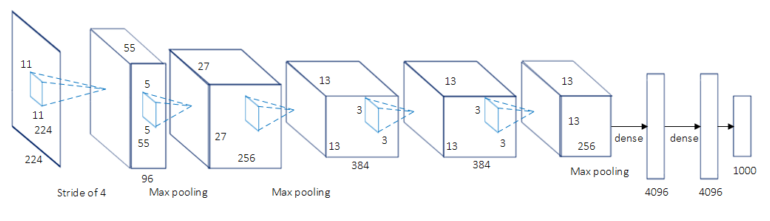
\includegraphics[width=0.7\linewidth]{fig/alexnet.png}
    \captionsource{AlexNet architecture}{\citet{Krizhevsky2012}}
    \label{fig:alexnet}
\end{figure}


\subsection{VGG}
The Visual Geometry Group (VGG) model was introduced by the Visual Geometry Group at Oxford University. In their paper, they propose multiple different architectural configurations with weight layers ranging from 13 - 16 layers deep. The most interesting is the model with 16 weight layers. It was submitted to ILSVRC 2013 and managed to get a top-5 test accuracy of 92.7\%. In \autoref{fig:vgg} we can see that the architecture makes use of more layers with small receptive fields rather than a few layers with large receptive fields.

\begin{figure}[H]
    \centering
    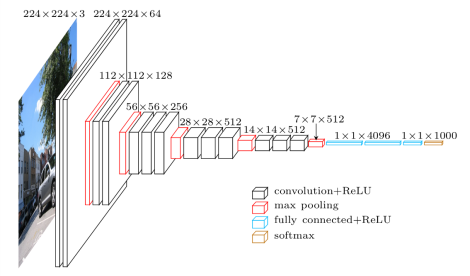
\includegraphics[width=0.7\linewidth]{fig/vgg16.png}
    \captionsource{VGG 16 architecture}{\citet{Cord}}
    \label{fig:vgg}
\end{figure}


\subsection{GoogLeNet}
This network won the 2014 ILSVRC challenge with a top-5 test accuracy of 93.3\%. The network introduced a new architectural concept called the \emph{inception} model (see \autoref{fig:inceptionmodule}). The model is essentially a new mini-network with a pooling operation, large convolution layers, and smaller convolution layers. They proposed the use of small 1x1 convolution layers to reduce the complexity before the large convolution layers to keep the parameters and computational cost under control. This showed an increase in speed ranging from 3-10x faster than similar networks without the inception module.

\begin{figure}[H]
    \centering
    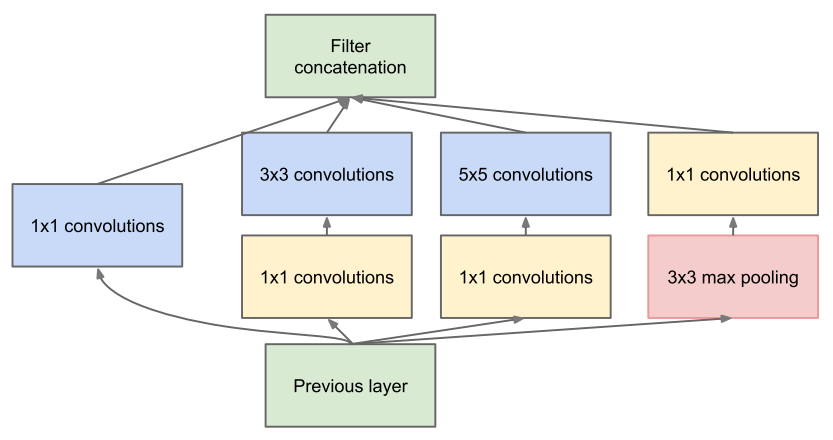
\includegraphics[width=0.7\linewidth]{fig/googlenet.png}
    \captionsource{Inception module}{\citet{Szegedy2014}}
    \label{fig:inceptionmodule}
\end{figure}


\subsection{ResNet}\label{subsection:resnet}
ResNet won the 2015 ILSVRC, with a top-5 test accuracy of 96.4\%. The network is known for its depth of 152 layers and a new kind of building block called residual block. The residual block contains two paths between the input and the output where one of the paths serve as a shortcut connection to the output (see \autoref{fig:residualblock}) essentially copying the input to the output layer. A big problem with very deep networks is that they are hard to optimize. When the depth of the network increases, the accuracy gets saturated. This is called \emph{degradation} and is the problem that the residual blocks are addressing by forcing the network to learn on top of already available input. 

\begin{figure}[H]
    \centering
    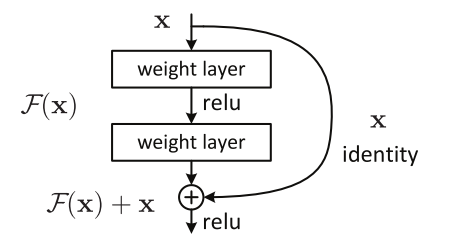
\includegraphics[width=0.5\linewidth]{fig/residual.png}
    \captionsource{Residual block.}{\citet{He2015}}
    \label{fig:residualblock}
\end{figure}


\subsection{CapsNet}
Released November 2017, this is a very recent advancement in neural networks. It introduces a new type of neural network based on \emph{capsules}. A capsule can be seen as a new type of neuron that instead of working on scalar values, encapsulates all the information about the state of the feature they are detecting in vector form.

It addresses the issue that CNN is not good at generalizing new viewpoints. They are good at generalizing to translation, but other affine transformations have shown to be difficult to learn. In the paper, the network is tested on the MNIST dataset. The results show a significant performance increase in the case of overlapping digits. 

Another important discovery is that the use of capsules makes the network capable of learning to state-of-the-art performance with a fraction of the data that a traditional CNN need.


\begin{figure}[H]
    \centering
    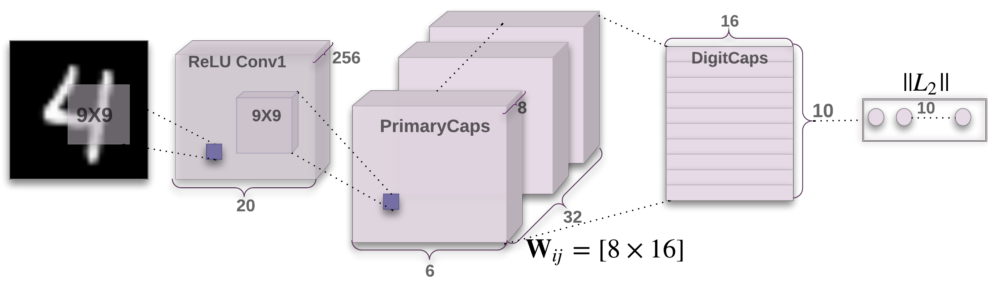
\includegraphics[width=0.7\linewidth]{fig/capsnet.png}
    \captionsource{CapsNet with 3 layers.}{\citet{Sabour2017}}
    \label{fig:capsnet}
\end{figure}


\section{Image segmentation}
Many of the previous network architectures described in \autoref{sec:important-architectures} are predicting labels of what the images contain and not where and what part of the image the labels are to be found in. Image segmentation is about assigning a class to each pixel with its enclosing object, also called dense predictions, so we need output from the networks that are spatial maps instead of classification scores. In this section, we will review important networks that are specialized in image segmentation. A benchmark often used for image segmentation is the PASCAL Visual Object Classes Challenge (VOC) \cite{Everingham2010}, that provides standardized image data sets for object class recognition. We will, therefore, evaluate the networks with the scores in VOC when applicable.


\subsection{FCN}
Fully Convolutional Network (FCN) by \citet{Long2014} can be seen as a common forerunner for semantic segmentation with convolutional networks \cite{Garcia-Garcia2017}. FCN adopted the contemporary deep classification nets AlexNet, VGG and GoogLeNet architectures we saw in \autoref{sec:important-architectures} to make dense predictions at the pixel level. It is important to note that they not only reused the architecture but used the pre-trained classification models as a starting point. The network replaced the fully-connected layers with convolutional ones, noting that the fully-connected layers could be seen as convolutional ones with kernels (filters) that cover the entire input region. This allowed segmentation maps to be generated from images of any size. Because of all the pooling operations in CNN, a technique called \emph{deconvolution} \cite{Zeiler2011} was used to upsample the coarse output to dense pixels. Deconvolutional layers can learn interpolation functions the same way the network learns weights. Skip connections similar to the ones we saw in ResNet, are also included to give the deeper layers higher resolution feature maps. It reached a score of 62.2 in the VOC2012 challenge. 


\subsection{SegNet}
SegNet by \citet{Badrinarayanan2015} uses an Encoder-Decoder architecture. One can also view FCN as this type of architecture, where the downsampling is the encoding part and the deconvolution is the decoder part. The difference between these networks is in the decoding part of the architecture. In SegNet more shortcut connections are added, however, instead of copying the input to the output of one layer, each upsampling layer corresponds to a max-pooling layer in the encoding part and the indices from the max-pooling layer is copied to the upsampling layer. This can be seen in \autoref{fig:segnet} where we see the blue lines as shortcut connections to the upsampling layers. The network was not benchmarked on VOC2012 in the paper but the leaderboard \cite{PASCALVOC2012a} shows that it reached a score of 59.9. 

\begin{figure}[H]
    \centering
    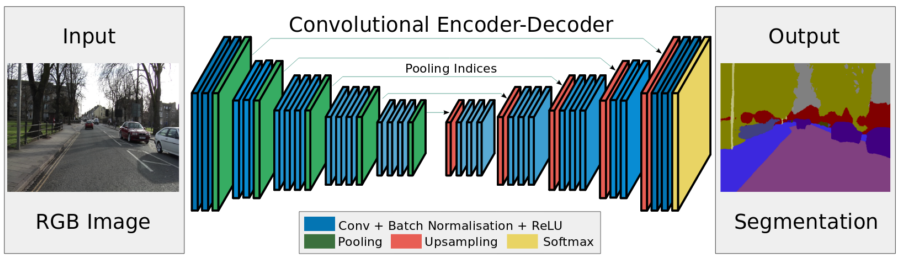
\includegraphics[width=0.7\linewidth]{fig/segnet.png}
    \captionsource{SegNet architecture.}{\citet{Badrinarayanan2015}}
    \label{fig:segnet}
\end{figure}


\subsection{Dilated Convolutions}
A problem with pooling layers is that they remove more context and resolution from the image the deeper we get into the network. For segmentation, we need contextual reasoning and full-resolution output and \citet{Yu2015} try to solve this problem with dilated convolution layers. Dilated convolution layers can increase the receptive field of a convolutional filter exponentially while the number of parameters grows linearly. This is illustrated in \autoref{fig:dilution} where we see that the receptive field,  indicated in green, grows exponentially compared to the parameters, indicated as red dots. The network showed state-of-the-art performance with a simpler architecture, based on VGG-16 \cite{Simonyan2014a} than the competition, scoring 71.3 in VOC2012 with their basic network.

\begin{figure}[H]
    \centering
    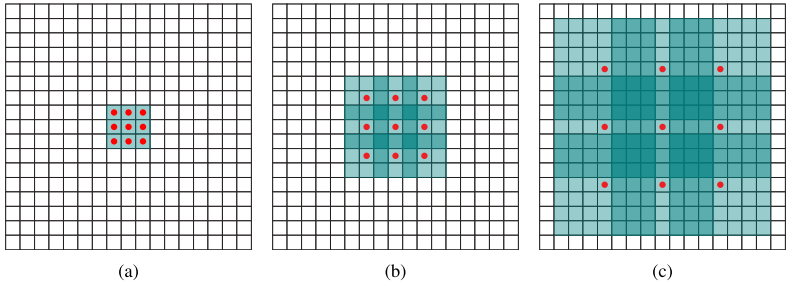
\includegraphics[width=0.7\linewidth]{fig/dilution.png}
    \captionsource{Diluted filters. (a) 1-dialted, (b) 2-dialated, (c) 3-dialated.  }{\citet{Yu2015}}
    \label{fig:dilution}
\end{figure}


\subsection{DeepLab (v1 \& v2)}
DeepLab v1 (2014) \cite{Chen2014} and DeepLab v2 (2016) \cite{Chen2016} both used dilated convolutions though they refer to them as \emph{atrous convolutions}. They use fully-connected Conditional Random Fields (CRF) to capture fine-grained details in images as proposed by \citet{Krahenbuhl2012a}. CRF can be used to combine the class scores from DCNN with the low-level information captured by the local interactions of pixels and edges \cite{Chen2014} and is used in DeepLab v1 as a post-processing method. As we can see in \autoref{fig:deeplab1} the effect of using CRF is significant in regards to detecting details in the image. DeepLab v1 used VGG-16 as a starting point for their architecture and got a score of 71.6 at VOC2012 beating the runner-up by a margin of 7.2\%. 

\begin{figure}[H]
    \centering
    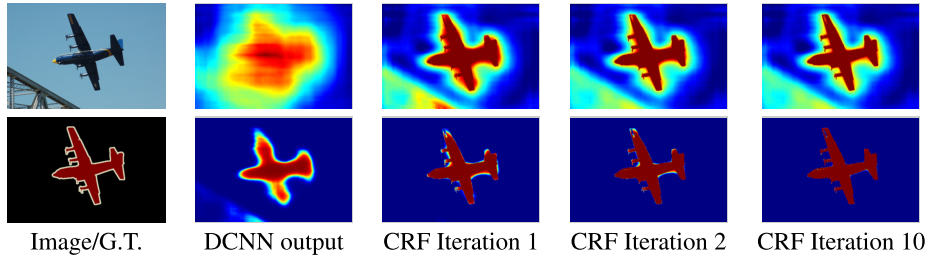
\includegraphics[width=0.7\linewidth]{fig/deeplab1.png}
    \captionsource{Score map (input before softmax) and belief map (output after softmax).  }{\citet{Chen2014}}
    \label{fig:deeplab1}
\end{figure}


DCNN can represent different object scales by training on datasets that contain objects of varying size. However explicitly accounting for scale can improve the networks ability to handle large and small objects \cite{Papandreou2015}. DeepLab v2 introduces a new technique to handle multivariate scale, called \emph{atrous spatial pyramid pooling} (ASPP). It uses multiple parallel atrous convolutional layers with different sampling rate/direction to improve the networks ability to deal with objects of different scale. DeepLab v2s best architecture used a pre-trained ResNet-101 (ResNet seen in \autoref{subsection:resnet}, that has 101 layers) with atrous convolutions, ASSP, and CRF that got a score of 79.7 at VOC2012.


\subsection{DeepLab v3}
In DeepLab v3 ,\citet{Chen2017a} introduce an improved model of ASSP that involves concatenation of image-level features, a 1x1 convolution and three 3x3 atrous convolutions with different rates as seen in \autoref{fig:deeplab3}.

\begin{figure}[H]
    \centering
    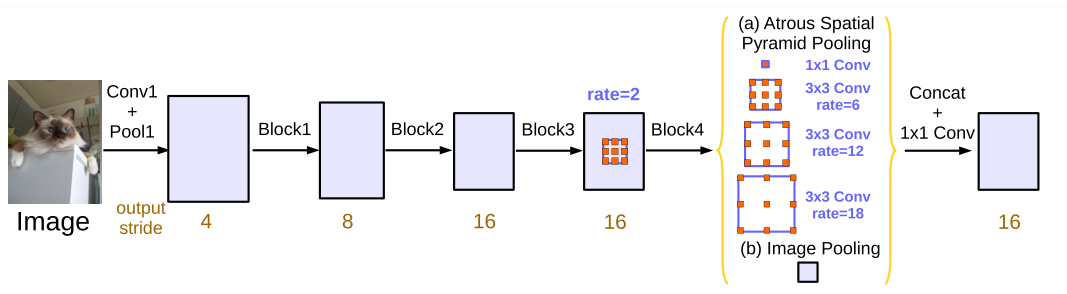
\includegraphics[width=0.8\linewidth]{fig/deeplab3.png}
    \captionsource{Improved version of ASSP, augmented with image-level features.  }{\citet{Chen2017a}}
    \label{fig:deeplab3}
\end{figure}

\emph{Cascading modules} was also proposed. A technique where the last ResNet block is duplicated multiple times and modified with atrous convolution Each block consists of three atrous convolution layers as seen in \autoref{fig:cascading}.

Both methods were tested, but the new ASSP performed better and was selected for use in the final model. Using a ResNet-101 pre-trained on ImageNet dataset, DeepLabv3 reached a performance of 85.7 on VOC2012. Using a ResNet-101 pre-trained on both ImageNet and JFT-300M dataset (internal dataset at Google with over 300M images \cite{Hinton2015}\cite{Sun2017}), DeepLabv3-JFT got a score of 86.9 on VOC2012 and became the leader of the competition.

\begin{figure}[H]
    \centering
    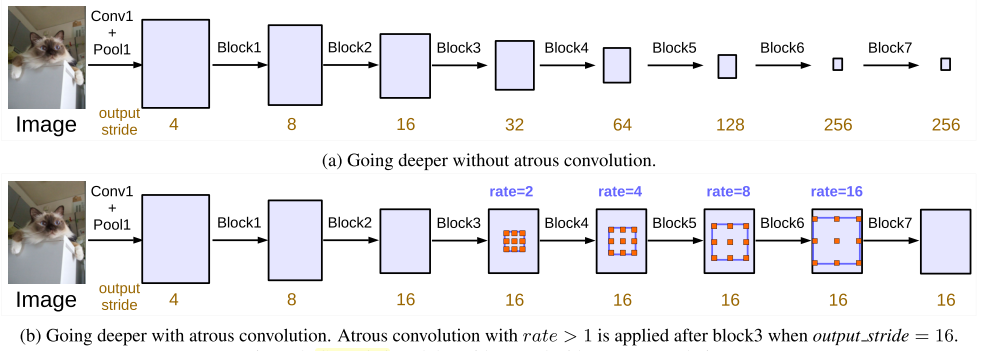
\includegraphics[width=0.8\linewidth]{fig/cascading.png}
    \captionsource{Cascaded modules.}{\citet{Chen2017a}}
    \label{fig:cascading}
\end{figure}




\chapter{Previous work - Rastermap Vectorization}
Image segmention has come a long way on images of normal everyday objects with deep CNNs. However none of the reviewed papers use their networks on raster maps. Not a lot of work has been done in regards to vectorization of raster maps using neural networks. However there has been a fair amount of research done on other techniques.

More work on satellite images.

Non artificial methods 

\section{Non-artifical intelligence methods}

\citeauthor{Leyk2010} presents a color image segmentation of raster maps from the \nth{19} century suffering from poor quality with a clustering technique using the local image plane, frequency domain an color space. The goal of the color image segmentation is to reduce the color values to fit the original colors used when printing the map. The method managed to segment lines, symbols and areas that belong to different color layers however there where still some minor classification errors that had to be solved manually.

In \cite{Iosifescu2016}, open-source solutions are used to vectorize historical maps from the \nth{19} century. Their procedure consists of five steps: Scanning of the map, georeferencing the map, pre-processing of an image to clean artifacts, automatic vectorization, automatic cleaning of the results. The authors note that the pre-processing step and scan quality are the most crucial for the performance of the vectorization and has to be customized for each set of raster maps. The pre-processing consist of RGB channel processing, conversion to binary images and cleaning. By processing the RGB channels in the image, different features on the map can be highlighted. An example of the building extraction can be seen in \autoref{fig:map-preprocessing}. 

\begin{figure}[H]
	\centering
	
\includegraphics[width=\linewidth]{fig/map-processing.png}
	\captionsource{From left to right: Original image, RBG processed, binary representation and cleaned}{\citeauthor{Iosifescu2016}\cite{Iosifescu2016}}
	\label{fig:map-preprocessing}
\end{figure}

The pre-processed image is then converted to vector format with Geospatial Data Abstraction Library\cite{OSGeo}(GDAL)'s polygonize and contour methods. The results are acceptable when taking the quality of the maps into consideration.

\citeauthor{Henderson} do semantic segmentation of raster maps with three different unsupervised algorithms: k-means, graph theoretic and expectation maximation. The maps have 6 color values and the segmentation is based on the knowledge of these and thus limits the application on more advanced maps.


\subsection{Multi stage system}
\cite{Oka2012}


\section{Artificial intelligence methods}

\subsection{VecNET}
(Maybe not even relevant because of bad quality of paper and use of ANN?)

VecNet proposed by \citeauthor{Karabork2008} in 2008 is one of few examples of vectorization of cartographic raster maps using a neural network. The authors present a three-step process consisting of thinning, line tracking with ANN and simplification. The main goal of the network is to find the critical points of objects, that is, to find breakage points of lines. They use an ANN with an input layer, a hidden layer and an output layer to classify. The training set is very small with only 16 samples. The output layer is a single vector with size 12, where the 8 first places represent an 8-way chain code of directions (the direction the line is following) and the last four represent a prediction of where the next pixel is going to be. It evaluates if the point is critical by checking if the last 8-way direction is different from the one currently calculated. If the point is critical, they store it.

The algorithm is tested on a single raster map only consisting of lines and does not perform better than a sparse pixel algorithm, but manages to get acceptable results according to the authors.

\subsection{Knowledge based system}
\cite{Lee2000}

\cite{Song2000}



\chapter{Discussion}


\chapter{Implementation}
\chapter{Conclusion}
DCNNs have shown great ability to do dense predictions of semantic labels in images with accuracy up to 86.9\% on the VOC2012 dataset. Huge datasets have been made for the training of these nets and data availability seems to be the biggest factor in success nowadays, but recent approaches such as CapsNet \cite{Sabour2017} try to lower the demand for data.

Some of the approaches using existing open source tools show interesting results in vectorization, but the need for uniform and similar maps does however limit the application when working with maps of different quality.

With the performance seen in the results of the DCNNs reviewed in this paper, there is no reason to believe that they should not be able to vectorize the zoning regulations as proposed. However, one of the biggest challenges found is the need to create a specific dataset. As seen in \autoref{chp:dataset} there is no simple way to know the location of the zoning area within the PDF, so a procedure needs to be done in order to fully automate the creation of the dataset. This needs to be investigated further in order to draw a conclusion regarding the feasibility of making such dataset.

If such dataset is created, either manually, automatically or by crowd sourcing, the work proposed in this paper could greatly speed up the process of vectorizing old zoning regulations by automating the whole process. Automation could yield substantial economic savings and an effort should be given to evaluating different methods in order to do so.

% Include more chapters as required.
%%=========================================
\appendix
% !TEX encoding = UTF-8 Unicode
%!TEX root = thesis.tex
% !TEX spellcheck = en-US
%%=========================================

\chapter{Acronyms}
\begin{description}
\item[FTA] Fault tree analysis
\item[MTTF] Mean time to failure
\item[RAMS] Reliability, availability, maintainability, and safety
\end{description}
% !TEX encoding = UTF-8 Unicode
%!TEX root = thesis.tex
% !TEX spellcheck = en-US
%%=========================================

\chapter{What to put in appendixes}
This is an example of an Appendix. You can write an Appendix in the same way as a chapter, with sections, subsections, and so on. An appendix may include list of code (in case you are programming), more details about results that you have presented in the report (could be a more complete  description of results, in case you decided to focus on the most important ones in the main report), supplementary information and descriptions you have found relating to the system you are analysing, such as drawings. You may discuss with your supervisor what are relevant information for appendixes.

%%=========================================
\section{Introduction}

%%=========================================
\subsection{More Details}
% Include more appendices as required.
%%=========================================
\bibliographystyle{apa}
\addcontentsline{toc}{chapter}{\bibname}
\bibliography{library}  
%%=========================================
%\include{vitae}         % Your curriculum Vitae     
%%=============================================

\end{document}
